\section{Análise preliminar}

Na análise teórica, considera-se o comportamento não linear do diodo e a capacidade de armazenamento do capacitor. Determina-se as equações que descrevem a relação entre a tensão de entrada e a tensão de saída do circuito, levando em conta os parâmetros do diodo e do capacitor. Com essas equações permite-se compreender como o circuito "grampeia" a tensão mínima em 0 V e como a forma e amplitude da onda de entrada afetam a tensão de saída.

\subsection{O circuito}

\begin{figure}[h]
    \centering
    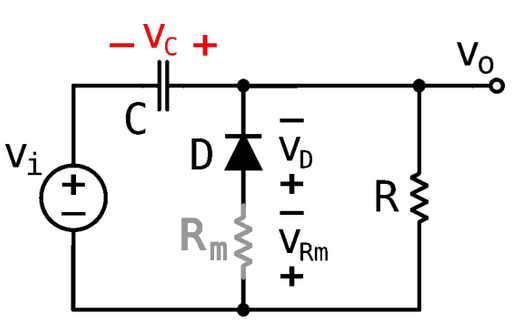
\includegraphics[width=1\columnwidth]{images/o_circuito.png}
    \caption{Circuito com diodo em configuração de grampeador.}
\end{figure}

\newpage
\subsection{Análise simbólica}

Faz-se a análise de cada estado do diodo separadamente, inicia-se com o diodo polarizado diretamente, e depois com este polarizado reversamente.

\subsubsection{Estado 1: Polarizacao direta}

\begin{figure}[h]
    \centering
    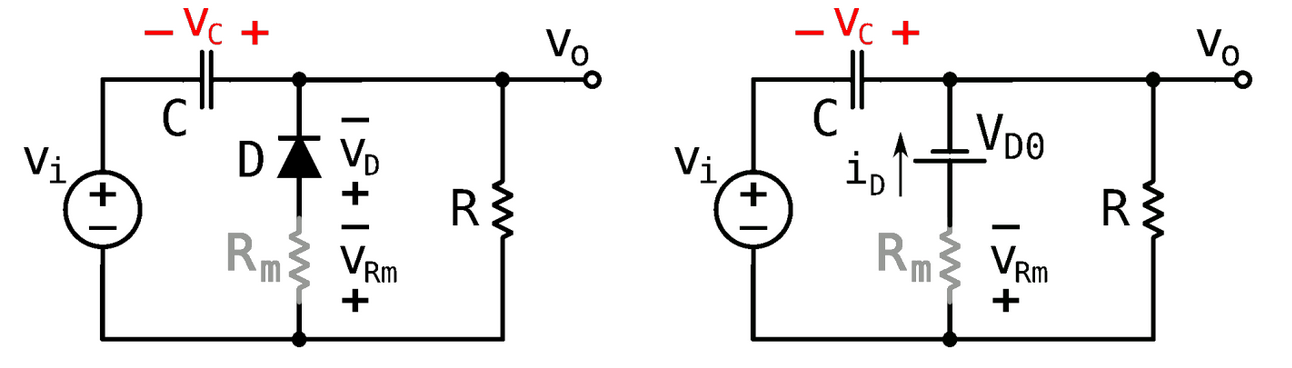
\includegraphics[width=1\columnwidth]{images/o_circuito_direto.png}
    \caption{Circuito grampeador de tensao em configuração de polarizacao direta.}
\end{figure}

Atinge-se este estado quando o diodo esta "ligado".

Neste caso tem-se restricoes

\begin{equation}
    \begin{aligned}
         & I_d > 0      \\
         & V_d = V_{D0}
    \end{aligned}
\end{equation}

Aplica-se a lei de Kirchhoff para o no $V_o$.

\begin{equation}
    \frac{V_o}{R} + \frac{V_o - ( - V_{D0})}{R_m} + C \deriv{V_c}{t} = 0
\end{equation}

Observa-se que:

\begin{equation}
    V_c = V_o - V_i
\end{equation}

\begin{equation}
    \deriv{V_c}{t} + \left( \frac{1}{R_m} + \frac{1}{R} \right) \frac{V_o}{C} = - \frac{V_{D0}}{R_m C}
\end{equation}

Rearranjando a equação:

\begin{equation}
    \deriv{V_c}{t} + \left( \frac{1}{R_m} + \frac{1}{R}\right) \frac{V_o}{C} = - \frac{V_{D0}}{R_m C}
\end{equation}

Como $V_c = V_o - V_i$: obtem-se:

\begin{equation}
    \label{eq:diff_eq1}
    \deriv{V_o}{t} + \frac{1}{C} \left(\frac{1}{R_m} + \frac{1}{R} \right) V_o = \deriv{V_i}{t} - \frac{V_{D0}}{R_m C}
\end{equation}
\\
A condicao inicial para  $V_o$ em funcao $V_{C0} = v(t=0)$ eh $V_o(0) = V_{C0} + V_i$.\\

Nesta pratica, faz-se duas premissas:

\begin{itemize}
    \item $R_m \ll R$. \\
    \item  $V_i$ eh uma onda quadrada de amplitude $\pm V_m$ e periodo $T_s$.
\end{itemize}

Da primeira premissa obtem-se:

\begin{equation}
    \frac{1}{R_m} + \frac{1}{R} \approx \frac{1}{R_m}
\end{equation}

E da segunda premissa, entre as transicoes entre $\pm V_m$ tem-se:

\begin{equation}
    \deriv{V_i}{t} = 0
\end{equation}

Pode-se entao simplificar a equacao \ref{eq:diff_eq1} como:

\begin{equation}
    \label{eq:diff_eq_estado1}
    \deriv{V_o}{t} + \frac{V_o}{R_m C}= - -\frac{V_{D0}}{R_m C}
\end{equation}

Com condicao inicial: $V_o(t = 0^{+}) = V_{C0} \pm V_m$.

\hfill

Tem-se solucao da equacao diferencial \ref{eq:diff_eq_estado1} como a soma da solucao particular e da solucao homogenea como:

\begin{equation}
    \tag*{Parte homogenea}
    \deriv{V_{oH}}{t} + \deriv{V_{oH}}{R_m C} = 0
\end{equation}

\begin{equation}
    \tag*{Solucao generica}
    V_{oH}(t) = K e^{-\frac{t}{R_m C}}
\end{equation}

Com $K$ determinado pelas condicoes iniciais.

Por substituicao determina-se que uma solucao particular pode ser obitda por:

\begin{equation}
    V_{oP}(t) = - V_{D0}
\end{equation}

Assim tem-se como solucao completa:

\begin{equation}
    \tag*{Solucao completa}
    \label{eq:solucao_completa1}
    V_o(t) = K e^{-\frac{t}{R_m C}} - V_{D0}
\end{equation}



